\section{Durchführung}%
\label{sec:Durchführung}
Die Debye-Scherrer-Aufnahmen werden nach der Filmmethode nach Straumanis angefertigt.

\subsection{Versuchsaufbau}%
\label{sub:versuchsaufbau}
Der prinzipielle Versuchsaufbau ist in Abbildung~\ref{fig:versuchsaufbau} dargestellt.
\begin{figure}
  \centering
  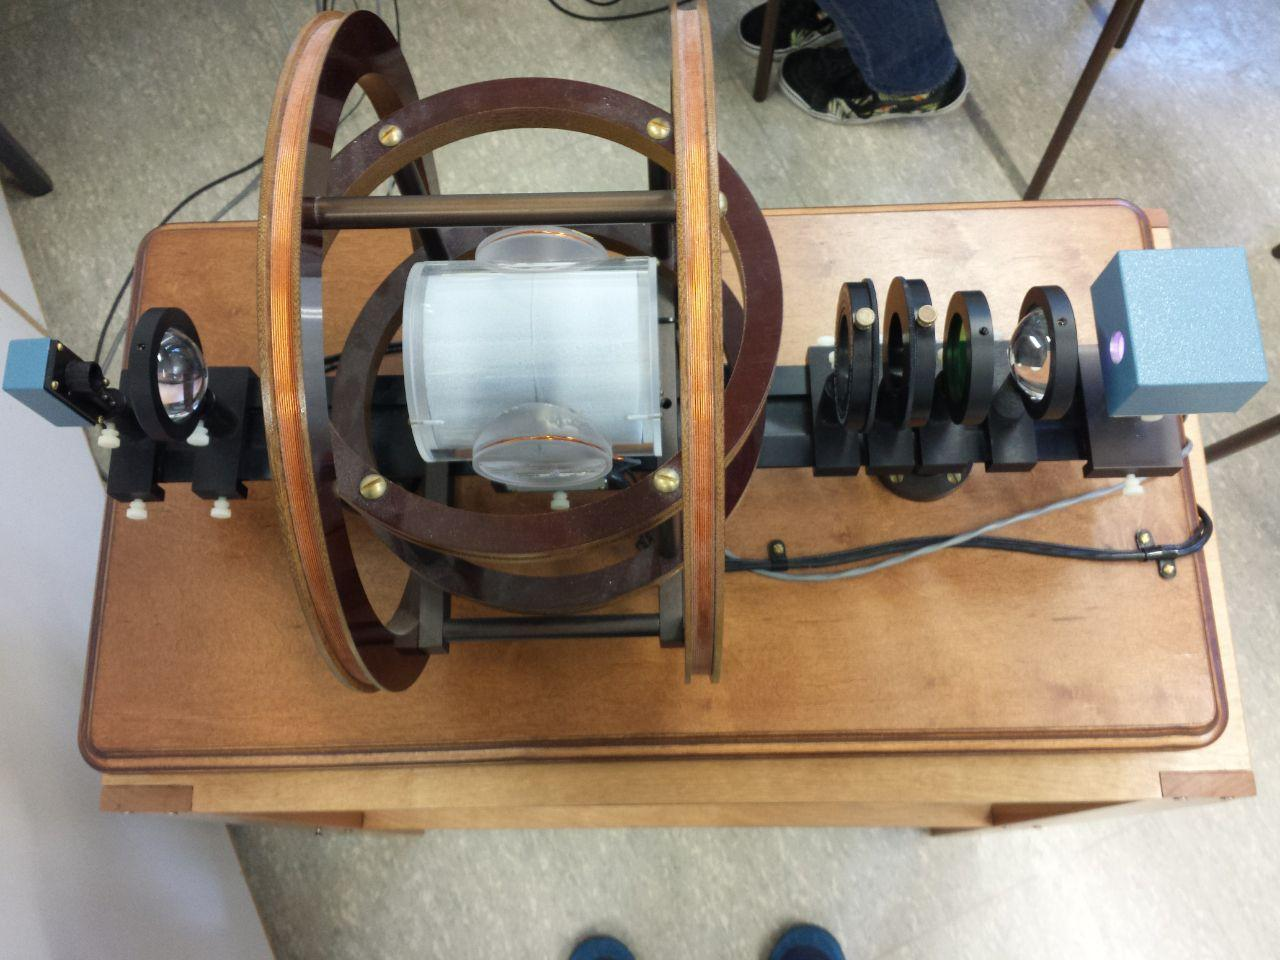
\includegraphics[width=0.8\linewidth]{build/versuchsaufbau.pdf}
  \caption{Prinzipielle Darstellung des Versuchsaufbaus.\cite{anleitung}}%
  \label{fig:versuchsaufbau}
\end{figure}

Ein Glasröhrchen mit einem Durchmesser von \SI{0.9}{\milli\meter} wird mit Vaseline bestrichen.
Die pulverisierte Probe wird außen auf das Röhrchen gebracht.

Die Probe ist in der Mitte einer runden Filmkamera befestigt.
Durch ein Kollimatorrohr wird die Röntgenstrahlung gebündelt.

Die gestreute Röntgenstrahlung schwärzt den Film beim Auftreffen.
Aufgrund der statistisch verteilten Anordnung in der pulverisierten Probe
ergeben die Streuungen der verschiedenen Gitterebenen Kreise auf dem Film,
die aufgrund der Maße des Filmstreifens als gekrümmte Linien zu sehen sind.

Die Kamera wird auf einer Schiene am Röntgengerät befestigt.
Es muss zum Starten des Versuchs eine Blende beseitigt werden und die Kamera
möglichst gut nach außen abgeschirmt werden.

Bevor die Messung gestartet wird, müssen alle möglichen Schalter auf Null gestellt werden.
Es wird eine Beschleunigungsspannung $U = \SI{40}{\kilo\volt}$ und ein
Anodenstrom $A = \SI{20}{\milli\ampere}$ eingestellt.
Die Messzeit wird über eine Stoppuhr eingestellt.


\subsection{Messung}%
\label{sub:messung}
Um eine zuverlässige Messung durchzuführen, muss die Probe justiert werden.
Die Probe wird durch den Ausgangskollimator mit einer Lampe belichtet,
sodass durch den Eingangskollimator hindurch geschaut werden kann.
Die Probe wird mittig im sichtbaren Bereich ausgerichtet.
Es wird darauf geachtet, dass sich während der Rotation der Probe diese nicht verschiebt.

Zuerst wird ein Probefilmstreifen mit einem unbeschichteten Glasrohr belichtet.
Die Messung dauert \SI{1}{\hour}.
Es wird eine gleichmäßige Schwärzung des Filmstreifens erwartet.

Die Messung mit \enquote{Probe 2} wird \SI{2}{\hour} belichtet.
Die Messung mit \enquote{Salz 2} wird \SI{4}{\hour} belichtet.
Hier werden deutlich erkennbare Linien erwartet.

\subsection{Fotoentwicklung}%
\label{sub:fotoentwicklung}
Die Filmstreifen müssen manuell entwickelt werden.
Hierfür muss unter dunklem Rotlicht gearbeitet werden!

Der belichtete Film wird \SI{15}{\minute} in einer Dose mit Entwickler geschwenkt,
danach \SI{1}{\minute} mit Wasser abgewaschen.
Der entwickelte Film wird \SI{1}{\minute} in einem Unterbrecherbad geschwenkt,
danach \SI{1}{\minute} mit Wasser abgewaschen.
Der unterbrochene Film wird \SI{5}{\minute} in einer Dose mit Fixier gelegt,
danach \SI{5}{\minute} mit Wasser abgewaschen und anschließen \SI{30}{\minute} getrocknet.
